%----------------------------------------------------------------------------
\chapter{Korlátos modell ellenörző}
\label{sec:bmc}
%----------------------------------------------------------------------------
\section{Modell ellenőrzés}
%----------------------------------------------------------------------------
A \hyperref[sec:intro]{bevezetőben} már elmondtam miért fontos a modellellenőrzés, most inkább arról beszélek, hogy ez mit jelent az állapotgépek esetén. A \hyperref[fig:mcheck]{6. 1-es ábrán} látható a működés elve. A modellellenőrző tehát egy modell reprezentációt, és egy tulajdonságot kap bemenetként. És megadja, hogy teljesül-e az adott tulajdonság, vagy nem. Ilyenkor még egy példát is ad arra, amikor nem teljesül, amivel könnyen ellenőrizhetjük, hogy igaz volt-e. A másik esetben viszont, ha nem talál ellenpéldát akkor azt bebizonyítani, hogy valóban nincs, csak úgy lehet, ha a modellellenőrző működés közben bizonyítottan megtalál minden ellenpéldát. Ezt sokszor csak bizonyos korlátok mellett lehet biztosítani.

A tulajdonság, általában egy elérhetőségi vizsgálatot jelent\footnote{Elérhető-e egy állapot a kezdeti állapotkonfigurációból, úgy, hogy minden tranzíció elsütése érvényes, azaz teljesül az őrfeltétel}. A BMC\footnote{Bounded Model Checker, a korlátos modell ellenőrző rövid neve}-nél sincs ez másképp, ilyenkor az ellenpélda egy útvonal az elérni kívánt állapothoz\footnote{Mely tranzíciókat kell elsütni, milyen sorrendben}. Mivel azt szeretjük, ha a hibás esetekben van ellenpélda ez az állapot egy hibaállapot, ami a rendszer nem megfelelő működését jelzi.

A BMC a helyes működést, azaz hogy egy állapot biztosan nem érhető el nem tudja bizonyítani, mert végtelen ideig is tarthatna a futás ideje. Ezért inkább megfogalmaz egy korlátot: maximum K lépésből elérhető-e az adott állapot

\begin{figure}[!ht]
	\centering
	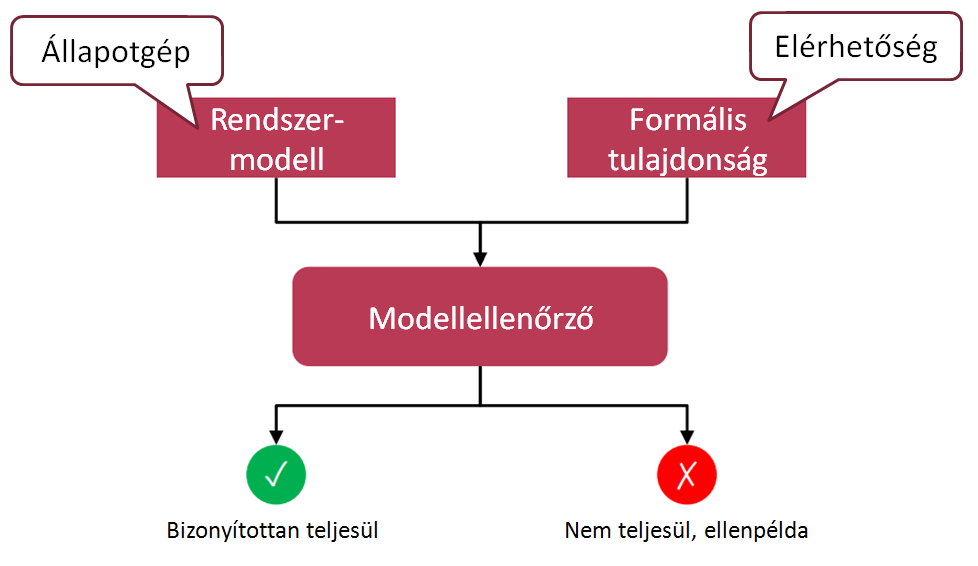
\includegraphics[width=74mm, keepaspectratio]{figures/altmc.png}\hspace{0cm}
	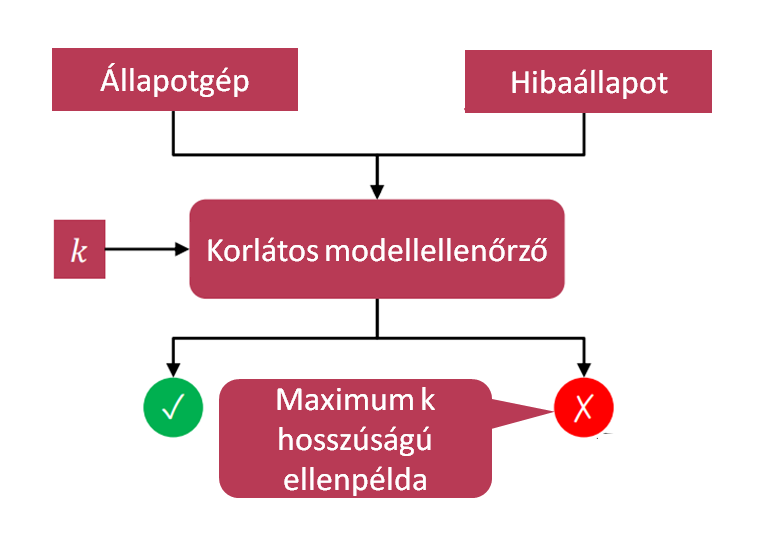
\includegraphics[width=74mm, keepaspectratio]{figures/bmc.png}
	\caption{Az általános ~ (balra) és a korlátos modellellenőrző (jobbra) működési elve}
	\label{fig:mcheck}
\end{figure}


%----------------------------------------------------------------------------
\section{A BMC menete}
%----------------------------------------------------------------------------
A korlátos modellellenőrző működése a \hyperref[fig:bmcfolyamat]{6.2-es ábrán} látható. A keresés egy szélességi gráf
bejárás az állapotkonfigurációkon ahol a k korlát mélységig megyünk. A hiba állapot olyan állapotgép konfigurációt jelent, ahol a hibaállapot aktív.

\begin{figure}[!ht]
	\centering
	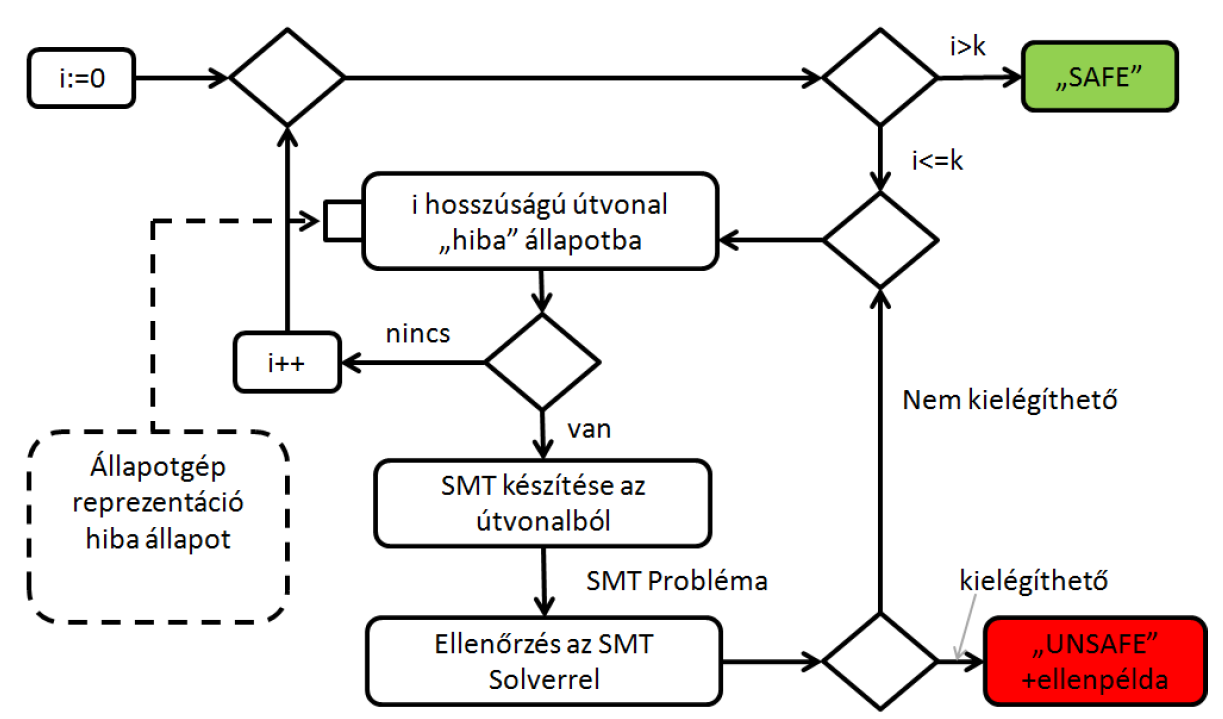
\includegraphics[width=150mm, keepaspectratio]{figures/bmcfolyamatmodell.png}
	\caption{A korlátos modellellenőrző folyamat modellje}
	\label{fig:bmcfolyamat}
\end{figure}

%----------------------------------------------------------------------------
\section{Az útvonal}
%----------------------------------------------------------------------------
A \verb+Path+ osztályt használom ennek a leírására. Tárolom az összes állapotgép konfigurációt az kiinduló állástól kezdve, és az útvonal során elsütött tranzíciókat.


\begin{lstlisting}[language=java,breaklines=true]
public boolean checkpath()
\end{lstlisting}

Azt ellenőrzi, hogy az útvonal helyes-e azaz minden egyes konfigurációból valóban jó konfigurációba léptünk és az elsütött tranzició elsüthető volt (a forrásállapota aktív volt)

\begin{lstlisting}[language=java,breaklines=true]
public StateConfiguration getResultConfiguration()
\end{lstlisting}

Az útvonal végigfutása utáni állapotkonfigurációt adja vissza


%----------------------------------------------------------------------------
\section{SMT Solver}
%----------------------------------------------------------------------------
Az SMT solver egy olyan eszköz, ami több aritmetikai kifejezést kapva, megtudja mondani, hogy ezek teljesülhetnek-e egyszerre. Ha igen akkor ad egy példa értéket az összes benne szereplő változóra, hogy azok kielégítsék mindegyik aritmetikai kifejezést.

Ezek most nekünk azért kellenek, mert az útvonalakon, a tranzíciókon lévő őrfeltételek is egy ilyen aritmetikai kifejezéshalmazt képeznek. 

A Theta projektben van egy interfész a Z3 solveréhez, ezt használtam.

Az \verb+SMTBuilder+ segéd osztályban csinálok az útvonalak segítségével SMT problémát, amit át tudok adni a solvernek.

\begin{lstlisting}[language=java,breaklines=true]
public SMTBuilder(final Path p) {
\end{lstlisting}
A segéd osztály egyszerűen létrehozható az útvonal alapján.


\begin{lstlisting}[language=java,breaklines=true]
public Collection<Expr<BoolType>> unfold()
\end{lstlisting}

Ezzel a függvénnyel hozzuk létre azt a listát, amit közvetlen átadhatunk a solvernek. 

Elsőre egyszerűnek tűnik, hiszen a tranzíciók, már ezt a formátumot használják az őrfeltételek tárolásához, de figyelemmel kell kísérni azt is, hogy az akciók során változhatnak a változó értékei -akár többször is-. Ennek a problémának a megoldásához van egy eszköz a Theta projekten belül (\verb+PathUtils+), ami pont ennek a "változó frissítésnek" ad implementációt. Itt válik hasznossá, hogy az \hyperref[sec:stateconfig]{állapotgép konfigurációkban tároljuk az összes akciót, ami a kezdeti állapothoz képest történt}.

%----------------------------------------------------------------------------
\section{BoundedChecker}
%----------------------------------------------------------------------------
Maga az ellenőrző osztály a \verb+BoundedChecker+.

\begin{lstlisting}[language=java,breaklines=true]
public BoundedChecker(final Sc chart, final int K, final State errorState)
\end{lstlisting}

Bemenetként egy állapotgépet várunk, amin végezzük az ellenőrzést. Bekérünk egy K korlátot, ami megadja a maximum lépés számot, és persze maga a hiba állapotot is kell.

\begin{lstlisting}[language=java,breaklines=true]
	public SafetyStatus check()
\end{lstlisting}

Ezzel a függvénnyel lehet futtatni az ellenőrzést, egy \verb+SafetyStatus+ al tér vissza amiből kiolvasható, hogy biztonságos-e, ha nem, akkor az ellenpéldát is ki lehet olvasni. Meghívja az \verb+algorithm+ függvényt

\begin{lstlisting}[language=java,breaklines=true]
public SafetyStatus algorithm(final Collection<Path> paths, final int deep) 
\end{lstlisting}

Egy rekurzív függvény ami, minden egyes lépésben növeli a mélységet (deep) és, minden útvonalból, (ami nem bukott már meg) létrehozza az összes lehetséges új útvonalakat. Ehhez elég az útvonal utolsó konfigurációján minden elsüthető tranzíciót elsütni.

Így biztosítjuk azt, hogy az összes lehetséges útvonalat megnézzük, aminek a hossza az inicializáláskor megadott maximumnál nem nagyobb. Tehát, ha nem találunk ellenpéldát akkor biztosan állíthatjuk, hogy nincs is.

A bizonyítás azért nem ennyire egyszerű, mert ugyan kipróbálunk minden lehetőséget, előfordulhat, hogy egy jó ellenpéldát nem fogadunk el, ez persze úgy lehet, ha például, rosszul építjük meg az SMT problémát és azt kapjuk, jogtalanul, hogy az útvonal nem teljesíthető.

További információ a \hyperref[sec:verifikacio]{verifikációs} résznél


